\clearpage
\section{Обзор литературы}

\subsection{Механизмы усложнения организации генома}

Увеличение разнообразия транскриптома и протеома у эукариот во многом достигается не только за счет классического эксцизионного сплайсинга, но и за счет ряда альтернативных механизмов обработки пре-мРНК.
В частности, альтернативный сплайсинг позволяет из одного транскрипта формировать несколько зрелых мРНК, отличающихся включением или исключением отдельных экзонов и участков~\cite{Mamon2019,Juneau2006}.

Одним из ключевых вариантов такого процесса является удержание интронов (intron retention, IR), когда интрон не удаляется и остается в составе зрелой мРНК.
Часто подобное сохранение интрона приводит к появлению в получившемся транскрипте преждевременных стоп-кодонов (premature termination codons, PTC), что запускает нонсенс-опосредованный распад (nonsense mediated mRNA decay, NMD).
Тем не менее в ряде случаев, последовательность интрона может включать специфические, функционально-значимые последовательности, такие как, например, конститутивный транспортный элемент (constitutive transport element, CTE).
Также интроны могут оказывать влияние на формирование устойчивой вторичной структуры, препятствующей связыванию факторов NMD, что позволяет транскриптам не подвергаться деградации.
Примечательно, что избегающие распада транскрипты способны даже участвовать в дальнейшем синтеза белка~\cite{Mamon2013,Jo2015,Kalyna2012}.

Кроме IR, альтернативный сплайсинг включает пропуск экзонов, использование альтернативных сайтов на 5'- и 3'-концах и кассетное включение/исключение блоков экзонов.
В совокупности эти механизмы значительно расширяют репертуар возможных транскриптов без необходимости увеличения числа генов.
Например, у многих многоклеточных организмов до 95\% генов подвергаются хотя бы одному типу альтернативного сплайсинга~\cite{Mamon2019}.
Для разных организмов продемонстрирована консервативность наличия транскрипта с сохраненным интроном, что подчеркивает эволюционную значимость интронов~\cite{Mamon2013}.

Таким образом, именно через комбинирование альтернативных способов сплайсинга, особенно удержания интронов, эукариоты получают мощный инструмент транскрипционной и белковой вариативности, что способствует адаптации и усложнению биологических процессов.


\subsection{Значимость интронов}

Традиционно интроны воспринимались лишь как ``ненужные`` вставки, но современные исследования убедительно показывают, что их функции выходят далеко за рамки простой ``пустоты``.
Во-первых, наличие интронных последовательностей может значительно усиливать уровень экспрессии генов.
Эксперименты на клеточных системах SV40, дрожжах \textit{Saccharomyces cerevisiae} и млекопитающих демонстрируют, что удаление ключевых интронов приводит к резкому снижению эффективности транскрипции и трансляции~\cite{Gruss1979,Juneau2006}.

Во-вторых, интроны влияют на чувствительность мРНК к нонсенс-опосредованному распаду.
Если интрон попадает в 5'- или 3'-UTR, его присутствие может менять архитектуру сплайсосомного комплекса, корректируя доступность PTC и, соответственно, баланс между сохранением транскрипта и его деградацией через NMD~\cite{Jo2015,Kalyna2012}.

Третья важная роль интронов заключается в транспорте мРНК из ядра в цитоплазму.
Долгое время считалось, что только полностью сплайсированные транскрипты эффективно экспортируются, однако при помощи FISH было показано, что РНК с сохраненными интронами также могут накапливаться в цитоплазме и функционировать там~\cite{Valencia2008,Jo2015,Roy2006}.
Это потребовало пересмотра классических представлений об экспорте мРНК.

Кроме регуляции экспрессии и транспорта, интроны участвуют в организации хроматиновой структуры.
Концевые последовательности интронов образуют участки с пониженной плотностью нуклеосом, что способствует более четкому разделению экзонов и облегчает процесс транскрипции~\cite{Schwartz2009}.

Наконец, интроны могут выполнять таксон- и тканеспецифические функции.
Так, первый интрон гена \textit{oskar} у Drosophila участвует в локализации мРНК в ооците, а длинные интронные вставки могут снижать интерференцию Хилла–Робертсона, улучшая кроссинговер в определенных регионах генома~\cite{Comeron2008}.
Результаты GWAS показывают, что однонуклеотидные варианты (single nucleotide variants, SNV) в интронных областях часто связаны с предрасположенностью к различным метаболическим и иммунным заболеваниям человека~\cite{Welter2014}.

Таким образом, интроны выполняют сложные регуляторные функции — от контроля уровня экспрессии до обеспечения оптимальной архитектуры хроматина и тканеспецифической регуляции транскриптов.


\subsection{Семейство генов \textit{Nxf}}

Гены \textit{Nxf} (nuclear export factor) названы по функции их наиболее известного представителя – \textit{Nxf1}, который обеспечивает экспорт большинства мРНК из ядра в цитоплазму.
Распространение этих генов наблюдается у всех эукариот группы Opisthokonta, однако их число и структурные особенности заметно различаются между таксонами.
У грибов обычно присутствует единственная копия \textit{Nxf}, тогда как в геномах растений и некоторых протистов такие гены могут отсутствовать полностью.
У животных же часто встречается от двух до пяти паралогов, что свидетельствует об активных дупликационных процессах в эволюции этого семейства~\cite{Mamon2013}.

Важнейшим элементом всех генов \textit{Nxf} является ``кассетный`` интрон, расположенный между двумя небольшими экзонами (110 и 37 нуклеотидов в каноническом варианте).
При альтернативном сплайсинге этот интрон может сохраняться в зрелой мРНК, неся внутри себя преждевременный стоп-кодон, возникающий за счет особенностей размеров упомянутых ранее экзонов.
Сохранению интрона может способствовать наличие определенных транспортных последовательностей, как у млекопитающих, или формирование устойчивой вторичной структуры.
В итоге такие транскрипты избегают NMD и могут кодировать укороченные, но функционально активные белки~\cite{Mamon2013,Golubkova2012}.

По основным характеристикам гена \textit{Nxf1} семейство можно разделить на 3 группы:

\begin{itemize}
  \item \textbf{Позвоночные.} У гена \textit{Nxf1} интрон располагается между 10-м и 11-м экзонами. Вставка содержит несколько консервативных мотивов, включая фрагмент, похожий на CTE, необходимый для экспорта частично сплайсированных РНК.
  \item \textbf{Дрозофилиды.} У представителей данного семейства кассетный интрон локализуется между 5-м и 6-м экзонами. В нем отсутствуют длинные гомологичные вставки, но присутствуют два тракта, обогащенные аденином (А) и формирующие прочную вторичную структуру, которая предположительно защищает транскрипт от деградации в ядре~\cite{Mamon2013}.
  \item \textbf{Нематоды.} У нематод интрон тоже располагается между 5-м и 6-м экзонами, но он гораздо короче и богат тимином (Т). Консервативные гомологи в таком интроне практически отсутствуют.
\end{itemize}

Эти различия отражают долгую эволюцию семейства \textit{Nxf}: от сравнительно простой короткой вставки у нематод до сложных CTE-подобных мотивов у позвоночных, подчеркивая ключевую роль кассетного интрона в посттранскрипционной регуляции~\cite{Mamon2013,Golubkova2012}.


\subsection{Структура и функции Nxf1 (гена и белка)}

Первоначально ген \textit{Nxf1} (известный как TAP у человека) был охарактеризован как ко-фактор белка Tip герпеса saimiri, отвечающий за экспорт несплайсированных и частично сплайсированных ретровирусных мРНК путем распознавания CTE-структуры в их последовательностях~\cite{Zolotukhin2001}.
У дрозофил этот ген также называют \textit{sbr}.

\begin{figure}[h] % here, top, bottom, page
    \centering
    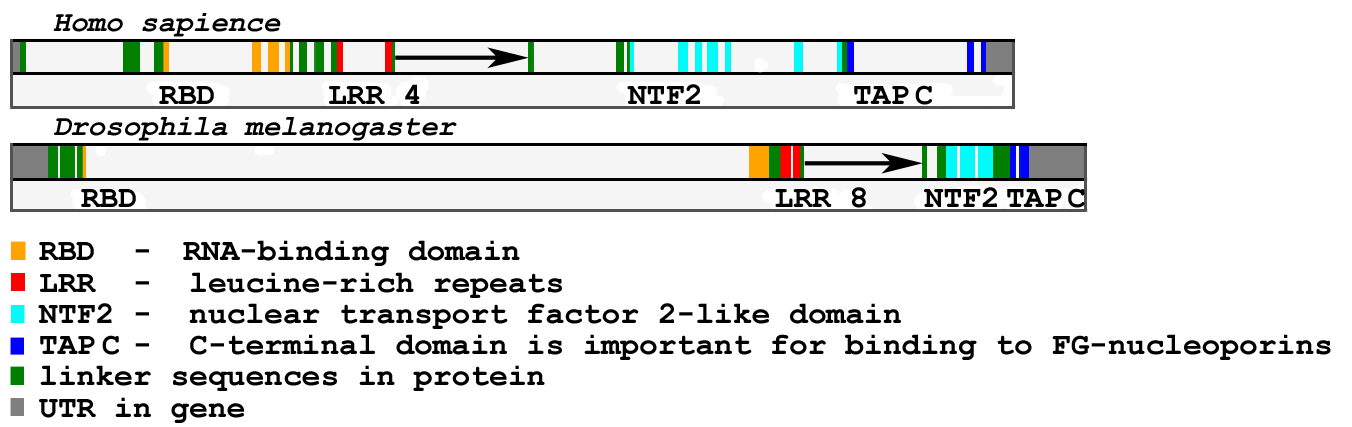
\includegraphics[width=0.9\textwidth]{images/dm_hs_nxf1_structure}
    \caption{Интрон-экзонная структура для генов \textit{Hs Nxf1} и \textit{Dm Nxf1}. Стрелки обозначают ``кассетный`` интрон. Цвета экзонов отображают белковые домены~\cite{Mamon2013}.}
    \label{fig:dm_hs_nxf1_structure}
\end{figure}

Белок Nxf1 включает несколько функциональных доменов (Рис.~\ref{fig:dm_hs_nxf1_structure}): RBD (домен связывания РНК), четыре лейцин-обогащенных повтора (LRR), NTF2-подобный домен, UBA-подобный домен и сигналы ядерной локализации в нетранслируемой области до экзонов.
В совокупности эти домены обеспечивают узнавание мРНК и взаимодействие с компонентами ядерного порового комплекса, делая \textit{Nxf1} основным экспортером мРНК~\cite{Herold2000,Mamon2013}.

Кассетный интрон, встроенный между сегментами RBD+LRR и NTF2L+UBA, выступает в роли ``переключателя``.
При его сохранении происходит синтез укороченных вариаций белка, обладающих специфической активностью~\cite{Mamon2013,Herold2000}.

Кроме классического транспорта мРНК, у \textit{Drosophila melanogaster} sbr выполняет органо- и тканеспецифические функции.
В сперматогенных клетках ген продуцирует укороченную форму sbr, необходимую для нормального сперматогенеза: без нее наблюдается резкое снижение фертильности~\cite{Ginanova2016}.
В центральной нервной системе sbr участвует в формировании границ между областями мозгового вещества зрительной системы, локализуясь в специфических нейронах и глиальных клетках и регулируя их ядерно–цитоплазматические комплексы~\cite{Mamon2021}.

Аналогичные эволюционно значимые особенности кассетного интрона отмечены у Chiroptera (Летучие мыши).
Сравнительный анализ продемонстрировал значимость кассетного интрона в эволюции гена \textit{Nxf1} у данной группы организмов~\cite{Bondaruk2022}.

Также в моей бакалаврской работе было показано, что структура ``консервативной кассеты`` является специфической для таксонов более низкого ранга у всех взятых в анализ артропод (89 видов), а интрон-содержащие транскрипты проанализированных дрозофилид (37 видов) формируют специфические вторичные структуры, имеющие А-обогащенные участки.

Таким образом, Nxf1 представляет собой пример многофункционального белка, чья доменная организация и альтернативные формы позволяют выполнять как основную задачу — экспорт мРНК, так и специализированные функции в разных тканях у разных таксонов.
